% This is a template for doing homework assignments in LaTeX, cribbed from M. Frenkel (NYU) and A. Hanhart (UW-Madison)

\documentclass{article} % This command is used to set the type of document you are working on such as an article, book, or presenation

\usepackage[margin=1in]{geometry} % This package allows the editing of the page layout. I've set the margins to be 1 inch. 

\usepackage{amsmath, amsfonts}  % The first package allows the use of a large range of mathematical formula, commands, and symbols.  The second gives some useful mathematical fonts.

\usepackage{graphicx}  % This package allows the importing of images
\usepackage{float} % more forced image positions

\usepackage{datetime}

%This allows us to use the theorem and proof environment 
\usepackage{amsthm}
\theoremstyle{plain}
\newtheorem*{theorem*}{Theorem}
\newtheorem{theorem}{Theorem}
\theoremstyle{definition}
\newtheorem*{definition*}{Definition}

%Custom commands.  
\newcommand{\abs}[1]{\left\lvert #1 \right\rvert} %absolute value command

%Custom symbols
\newcommand{\Rb}{\mathbb{R}}




\begin{document}

\begin{center}
    \Large{
        \textbf{Assignment \#3}

        UW-Madison MATH 421
    }
    
    \vspace{5pt}
        
    \normalsize{
        GEOFF YOERGER

        \usdate
        \formatdate{16}{2}{2021}
    }
    
    \vspace{15pt}
\end{center}


\noindent\fbox{\textbf{Exercise \#1:}} Sketch the set of all points $(x,y)$ in the plane satisfying 


\begin{figure}[H]
    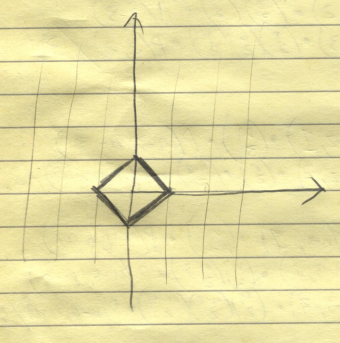
\includegraphics[width=200px]{diamond.png}
    \caption{$\abs{x}+\abs{y}=1$: A diamond}
\end{figure}
\begin{figure}[H]
    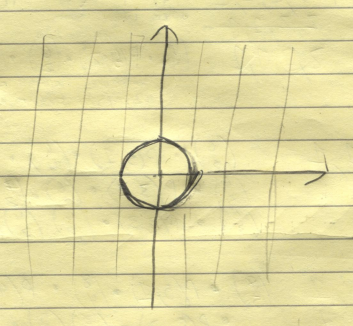
\includegraphics[width=200px]{circle.png}
    \caption{$x^2 + y^2 =1$: A circle}
\end{figure}
\begin{figure}[H]
    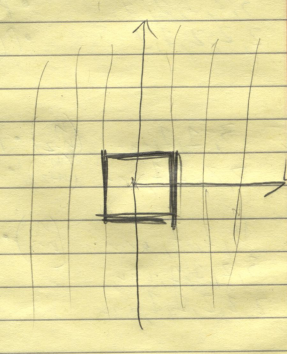
\includegraphics[width=200px]{square.png}
    \caption{$\max\{ \abs{x}, \abs{y} \} = 1$: A square}
\end{figure}

\vspace*{12pt}  %This adds some vertical space. 

\noindent\fbox{\textbf{Exercise \#2:}} Following the instructions on the previous problem: Spivak, Chapter 4, Problem 17 (i) and (ii). 

\begin{figure}[H]
    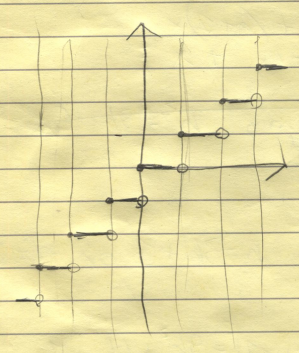
\includegraphics[width=200px]{steps.png}
    \caption{$f(x) = \left \lfloor {x} \right \rfloor$: Steps}
\end{figure}
\begin{figure}[H]
    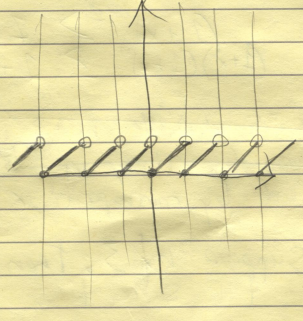
\includegraphics[width=200px]{sawteeth.png}
    \caption{$f(x) = x - \left \lfloor {x} \right \rfloor$: Sawteeth}
\end{figure}

\vspace*{12pt}  %This adds some vertical space. 


\noindent\fbox{\textbf{Exercise \#3:}} Prove, using only the definition, that $\lim_{x \rightarrow 3} 5x = 15$. 

\begin{proof} 

\end{proof} 

\noindent\fbox{\textbf{Exercise \#4:}} Prove, using only the definition, that $\lim_{x \rightarrow 2} x^2+2x = 8$. 

\begin{proof} 

\end{proof} 

\noindent\fbox{\textbf{Exercise \#5:}} Prove the following theorem: 

\begin{theorem*} If $x$ and $y$ are numbers, then $\abs{\abs{x}-\abs{y}} \leq \abs{x-y}$. 
\end{theorem*}

\begin{proof} (Hint: use a previous HW problem)

\end{proof} 


\noindent\fbox{\textbf{Exercise \#6:}} Spivak, Chapter 5,  16 (a)

\begin{proof} 

\end{proof} 

\noindent\fbox{\textbf{Exercise \#7:}} Spivak, Chapter 5, Problem 12 (a) 

\begin{proof} (Hint: a proof by contradiction can work)

\end{proof} 


\noindent\fbox{\textbf{Exercise \#8:}} Spivak, Chapter 5, Problem 37 (a) 

\begin{proof} 

\end{proof} 




    





    
    
\end{document}
